\documentclass{ximera}

\outcome{Use limits to find the slope of the tangent line at a point.}
\outcome{Understand the definition of the derivative at a point.}
\outcome{Compute the derivative of a function at a point.}
\outcome{Estimate the slope of the tangent line graphically.}
\outcome{Write the equation of the tangent line to a graph at a given point.}
\outcome{Recognize and distinguish between secant and tangent lines.}
\outcome{Recognize different notation for the derivative.}
\outcome{Recognize the the tangent line as a local approximation for a
  differentiable function.}

%\usepackage{todonotes}

\newcommand{\todo}{}

\usepackage{tkz-euclide}
\tikzset{>=stealth} %% cool arrow head
\tikzset{shorten <>/.style={ shorten >=#1, shorten <=#1 } } %% allows shorter vectors

\usepackage{tkz-tab}  %% sign charts
\usetikzlibrary{decorations.pathreplacing} 

\usetikzlibrary{backgrounds} %% for boxes around graphs
\usetikzlibrary{shapes,positioning}  %% Clouds and stars
\usetikzlibrary{matrix} %% for matrix
\usepgfplotslibrary{polar} %% for polar plots
\usetkzobj{all}
\usepackage[makeroom]{cancel} %% for strike outs
%\usepackage{mathtools} %% for pretty underbrace % Breaks Ximera
\usepackage{multicol}

\usepackage{polynom}



\usepackage[many]{tcolorbox}  %% for titled boxes
\newtcolorbox{xbox}[1]{%
    tikznode boxed title,
    enhanced,
    arc=0mm,
    interior style={white},
    attach boxed title to top center= {yshift=-\tcboxedtitleheight/2},
    fonttitle=\bfseries,
    colbacktitle=white,coltitle=black,
    boxed title style={size=normal,colframe=white,boxrule=0pt},
    title={#1}}


\usepackage{array}
\setlength{\extrarowheight}{+.1cm}   
\newdimen\digitwidth
\settowidth\digitwidth{9}
\def\divrule#1#2{
\noalign{\moveright#1\digitwidth
\vbox{\hrule width#2\digitwidth}}}





\newcommand{\RR}{\mathbb R}
\newcommand{\R}{\mathbb R}
\newcommand{\N}{\mathbb N}
\newcommand{\Z}{\mathbb Z}

%\renewcommand{\d}{\,d\!}
\renewcommand{\d}{\mathop{}\!d}
\newcommand{\dd}[2][]{\frac{\d #1}{\d #2}}
\newcommand{\pp}[2][]{\frac{\partial #1}{\partial #2}}
\renewcommand{\l}{\ell}
\newcommand{\ddx}{\frac{d}{\d x}}
\newcommand{\ddt}{\frac{d}{\d t}}

\newcommand{\zeroOverZero}{\ensuremath{\boldsymbol{\tfrac{0}{0}}}}
\newcommand{\inftyOverInfty}{\ensuremath{\boldsymbol{\tfrac{\infty}{\infty}}}}
\newcommand{\zeroOverInfty}{\ensuremath{\boldsymbol{\tfrac{0}{\infty}}}}
\newcommand{\zeroTimesInfty}{\ensuremath{\small\boldsymbol{0\cdot \infty}}}
\newcommand{\inftyMinusInfty}{\ensuremath{\small\boldsymbol{\infty - \infty}}}
\newcommand{\oneToInfty}{\ensuremath{\boldsymbol{1^\infty}}}
\newcommand{\zeroToZero}{\ensuremath{\boldsymbol{0^0}}}
\newcommand{\inftyToZero}{\ensuremath{\boldsymbol{\infty^0}}}



\newcommand{\numOverZero}{\ensuremath{\boldsymbol{\tfrac{\#}{0}}}}
\newcommand{\dfn}{\textbf}
%\newcommand{\unit}{\,\mathrm}
\newcommand{\unit}{\mathop{}\!\mathrm}
\newcommand{\eval}[1]{\bigg[ #1 \bigg]}
\newcommand{\seq}[1]{\left( #1 \right)}
\renewcommand{\epsilon}{\varepsilon}
\renewcommand{\iff}{\Leftrightarrow}

\DeclareMathOperator{\arccot}{arccot}
\DeclareMathOperator{\arcsec}{arcsec}
\DeclareMathOperator{\arccsc}{arccsc}
\DeclareMathOperator{\si}{Si}
\DeclareMathOperator{\proj}{proj}
\DeclareMathOperator{\scal}{scal}


\newcommand{\tightoverset}[2]{% for arrow vec
  \mathop{#2}\limits^{\vbox to -.5ex{\kern-0.75ex\hbox{$#1$}\vss}}}
\newcommand{\arrowvec}[1]{\tightoverset{\scriptstyle\rightharpoonup}{#1}}
\renewcommand{\vec}{\mathbf}
\newcommand{\veci}{\vec{i}}
\newcommand{\vecj}{\vec{j}}
\newcommand{\veck}{\vec{k}}
\newcommand{\vecl}{\boldsymbol{\l}}

\newcommand{\dotp}{\bullet}
\newcommand{\cross}{\boldsymbol\times}
\newcommand{\grad}{\boldsymbol\nabla}
\newcommand{\divergence}{\grad\dotp}
\newcommand{\curl}{\grad\cross}
%\DeclareMathOperator{\divergence}{divergence}
%\DeclareMathOperator{\curl}[1]{\grad\cross #1}


\colorlet{textColor}{black} 
\colorlet{background}{white}
\colorlet{penColor}{blue!50!black} % Color of a curve in a plot
\colorlet{penColor2}{red!50!black}% Color of a curve in a plot
\colorlet{penColor3}{red!50!blue} % Color of a curve in a plot
\colorlet{penColor4}{green!50!black} % Color of a curve in a plot
\colorlet{penColor5}{orange!80!black} % Color of a curve in a plot
\colorlet{fill1}{penColor!20} % Color of fill in a plot
\colorlet{fill2}{penColor2!20} % Color of fill in a plot
\colorlet{fillp}{fill1} % Color of positive area
\colorlet{filln}{penColor2!20} % Color of negative area
\colorlet{fill3}{penColor3!20} % Fill
\colorlet{fill4}{penColor4!20} % Fill
\colorlet{fill5}{penColor5!20} % Fill
\colorlet{gridColor}{gray!50} % Color of grid in a plot

\newcommand{\surfaceColor}{violet}
\newcommand{\surfaceColorTwo}{redyellow}
\newcommand{\sliceColor}{greenyellow}




\pgfmathdeclarefunction{gauss}{2}{% gives gaussian
  \pgfmathparse{1/(#2*sqrt(2*pi))*exp(-((x-#1)^2)/(2*#2^2))}%
}


%%%%%%%%%%%%%
%% Vectors
%%%%%%%%%%%%%

%% Simple horiz vectors
\renewcommand{\vector}[1]{\left\langle #1\right\rangle}


%% %% Complex Horiz Vectors with angle brackets
%% \makeatletter
%% \renewcommand{\vector}[2][ , ]{\left\langle%
%%   \def\nextitem{\def\nextitem{#1}}%
%%   \@for \el:=#2\do{\nextitem\el}\right\rangle%
%% }
%% \makeatother

%% %% Vertical Vectors
%% \def\vector#1{\begin{bmatrix}\vecListA#1,,\end{bmatrix}}
%% \def\vecListA#1,{\if,#1,\else #1\cr \expandafter \vecListA \fi}

%%%%%%%%%%%%%
%% End of vectors
%%%%%%%%%%%%%

%\newcommand{\fullwidth}{}
%\newcommand{\normalwidth}{}



%% makes a snazzy t-chart for evaluating functions
%\newenvironment{tchart}{\rowcolors{2}{}{background!90!textColor}\array}{\endarray}

%%This is to help with formatting on future title pages.
\newenvironment{sectionOutcomes}{}{} 



%% Flowchart stuff
%\tikzstyle{startstop} = [rectangle, rounded corners, minimum width=3cm, minimum height=1cm,text centered, draw=black]
%\tikzstyle{question} = [rectangle, minimum width=3cm, minimum height=1cm, text centered, draw=black]
%\tikzstyle{decision} = [trapezium, trapezium left angle=70, trapezium right angle=110, minimum width=3cm, minimum height=1cm, text centered, draw=black]
%\tikzstyle{question} = [rectangle, rounded corners, minimum width=3cm, minimum height=1cm,text centered, draw=black]
%\tikzstyle{process} = [rectangle, minimum width=3cm, minimum height=1cm, text centered, draw=black]
%\tikzstyle{decision} = [trapezium, trapezium left angle=70, trapezium right angle=110, minimum width=3cm, minimum height=1cm, text centered, draw=black]


\title[Dig-In:]{The definition of the derivative} 

\begin{document}
\begin{abstract}
We compute the instantaneous growth rate by computing the limit of
average growth rates.
\end{abstract}
\maketitle


Given a function, it is often useful to know the rate at which the
function changes. To give you a feeling why this is true, consider the
following:
\begin{itemize}
\item If $s(t)$ represents the \dfn{displacement} (position relative to an
  origin) of an object with respect to time, the rate of change gives
  the \dfn{velocity} of the object.
\item If $v(t)$ represents the \dfn{velocity} of an object with respect to
  time, the rate of change gives the \dfn{acceleration} of the object.
\item If $R(x)$ represents the revenue generated by selling $x$
  objects, the rate of change gives us the \dfn{marginal revenue},
  meaning the additional revenue generated by selling one additional
  unit. Note, there is an implicit assumption that $x$ is quite large
  compared to $1$.
\item If $C(x)$ represents the cost to produce $x$ objects, the rate
  of change gives us the \dfn{marginal cost}, meaning the
  additional cost generated by selling one additional unit. Again,
  there is an implicit assumption that $x$ is quite large compared to
  $1$.
\item If $P(x)$ represents the profit gained by selling $x$ objects,
  the rate of change gives us the \dfn{marginal profit}, meaning
  the additional cost generated by selling one additional unit. Again,
  there is an implicit assumption that $x$ is quite large compared to
  $1$.
\item The rate of change of a function can help us approximate a
  complicated function with a simple function.
\item The rate of change of a function can be used to help us solve
  equations that we would not be able to solve via other methods.
\end{itemize}



\section{From slopes of secant lines to slopes of tangent lines}

You've been computing average rates of change for a while now, the
computation is simply
\[
\frac{\text{change in the function}}{\text{change in the input to the
    function}}.
\]
However, the question remains: Given a function that represents an
amount, how exactly does one find the function that will give the
instantaneous rate of change? Recall that the instantaneous rate of change
of a line is the slope of the line.  Hence the instantaneous rate of
change of a function is the slope of the tangent line. For now,
consider the following informal definition of a \textit{tangent line}:
\begin{quote}\index{tangent line}
Given a function $f$ and a number $a$ in the domain of $f$, if one can ``zoom in''
on the graph at $(a, f(a))$ sufficiently so that it appears to be a straight line,
then that line is the \dfn{tangent line} to $f(x)$ at the point $(a,f(a))$.
\end{quote}
We illustrate this informal definition with the following diagram:
\begin{image}
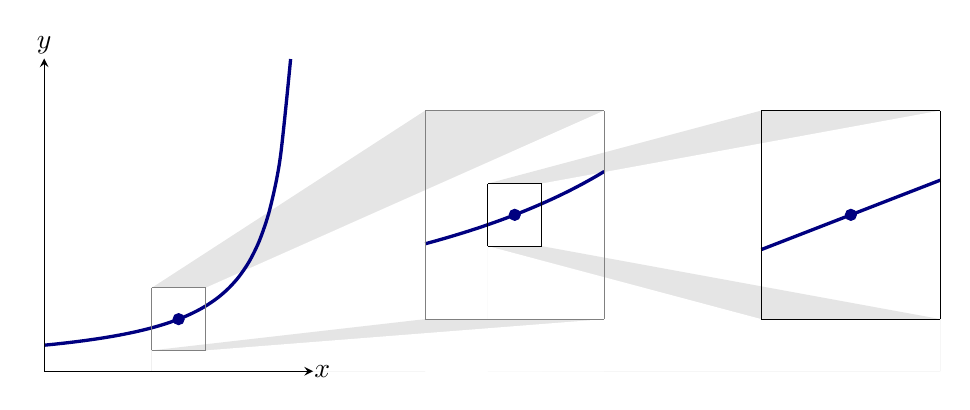
\begin{tikzpicture}
  \begin{axis}[
            domain=0:6, range=0:7,
            ymin=-.2,ymax=7,
            width=6in,
            height=2.5in, %% Hard coded height! Moreover this effects the aspect ratio of the zoom--sort of BAD
            axis lines=none,
          ]   
          \addplot [draw=none, fill=textColor!10!background] plot coordinates {(.8,1.6) (2.834,5)} \closedcycle; %% zoom fill
          \addplot [draw=none, fill=textColor!10!background] plot coordinates {(2.834,5) (4.166,5)} \closedcycle; %% zoom fill
          \addplot [draw=none, fill=background] plot coordinates {(1.2,1.6) (4.166,5)} \closedcycle; %% zoom fill
          \addplot [draw=none, fill=background] plot coordinates {(.8,1.6) (1.2,1.6)} \closedcycle; %% zoom fill

          \addplot [draw=none, fill=textColor!10!background] plot coordinates {(3.3,3.6) (5.334,5)} \closedcycle; %% zoom fill
          \addplot [draw=none, fill=textColor!10!background] plot coordinates {(5.334,5) (6.666,5)} \closedcycle; %% zoom fill
          \addplot [draw=none, fill=background] plot coordinates {(3.7,3.6) (6.666,5)} \closedcycle; %% zoom fill
          \addplot [draw=none, fill=background] plot coordinates {(3.3,3.6) (3.7,3.6)} \closedcycle; %% zoom fill
          
          \addplot [draw=none, fill=textColor!10!background] plot coordinates {(3.7,2.4) (6.666,1)} \closedcycle; %% zoom fill
          \addplot [draw=none, fill=textColor!10!background] plot coordinates {(3.3,2.4) (3.7,2.4)} \closedcycle; %% zoom fill
          \addplot [draw=none, fill=background] plot coordinates {(3.3,2.4) (5.334,1)} \closedcycle; %% zoom fill          
          \addplot [draw=none, fill=background] plot coordinates {(5.334,1) (6.666,1)} \closedcycle; %% zoom fill
          

          \addplot [draw=none, fill=textColor!10!background] plot coordinates {(.8,.4) (2.834,1)} \closedcycle; %% zoom fill
          \addplot [draw=none, fill=textColor!10!background] plot coordinates {(2.834,1) (4.166,1)} \closedcycle; %% zoom fill
          \addplot [draw=none, fill=background] plot coordinates {(1.2,.4) (4.166,1)} \closedcycle; %% zoom fill
          \addplot [draw=none, fill=background] plot coordinates {(.8,.4) (1.2,.4)} \closedcycle; %% zoom fill

          \addplot[very thick,penColor, smooth,domain=(0:1.833)] {-1/(x-2)};
          \addplot[very thick,penColor, smooth,domain=(2.834:4.166)] {3.333/(2.050-.3*x)-0.333}; %% 2.5 to 4.333
          %\addplot[very thick,penColor, smooth,domain=(5.334:6.666)] {11.11/(1.540-.09*x)-8.109}; %% 5 to 6.833
          \addplot[very thick,penColor, smooth,domain=(5.334:6.666)] {x-3}; %% 5 to 6.833
          
          \addplot[color=penColor,fill=penColor,only marks,mark=*] coordinates{(1,1)};  %% point to be zoomed
          \addplot[color=penColor,fill=penColor,only marks,mark=*] coordinates{(3.5,3)};  %% zoomed pt 1
          \addplot[color=penColor,fill=penColor,only marks,mark=*] coordinates{(6,3)};  %% zoomed pt 2

          \addplot [->,textColor] plot coordinates {(0,0) (0,6)}; %% axis
          \addplot [->,textColor] plot coordinates {(0,0) (2,0)}; %% axis
          
          \addplot [textColor!50!background] plot coordinates {(.8,.4) (.8,1.6)}; %% box around pt
          \addplot [textColor!50!background] plot coordinates {(1.2,.4) (1.2,1.6)}; %% box around pt
          \addplot [textColor!50!background] plot coordinates {(.8,1.6) (1.2,1.6)}; %% box around pt
          \addplot [textColor!50!background] plot coordinates {(.8,.4) (1.2,.4)}; %% box around pt
          
          \addplot [textColor!50!background] plot coordinates {(2.834,1) (2.834,5)}; %% zoomed box 1
          \addplot [textColor!50!background] plot coordinates {(4.166,1) (4.166,5)}; %% zoomed box 1
          \addplot [textColor!50!background] plot coordinates {(2.834,1) (4.166,1)}; %% zoomed box 1
          \addplot [textColor!50!background] plot coordinates {(2.834,5) (4.166,5)}; %% zoomed box 1

          \addplot [textColor] plot coordinates {(3.3,2.4) (3.3,3.6)}; %% box around zoomed pt
          \addplot [textColor] plot coordinates {(3.7,2.4) (3.7,3.6)}; %% box around zoomed pt
          \addplot [textColor] plot coordinates {(3.3,3.6) (3.7,3.6)}; %% box around zoomed pt
          \addplot [textColor] plot coordinates {(3.3,2.4) (3.7,2.4)}; %% box around zoomed pt

          \addplot [textColor] plot coordinates {(5.334,1) (5.334,5)}; %% zoomed box 2
          \addplot [textColor] plot coordinates {(6.666,1) (6.666,5)}; %% zoomed box 2
          \addplot [textColor] plot coordinates {(5.334,1) (6.666,1)}; %% zoomed box 2
          \addplot [textColor] plot coordinates {(5.334,5) (6.666,5)}; %% zoomed box 2

          \node at (axis cs:2.2,0) [anchor=east] {$x$};
          \node at (axis cs:0,6.6) [anchor=north] {$y$};
        \end{axis}
\end{tikzpicture}

\end{image}
%% \todo{This image should be interactive.}




The \textit{derivative} of a function $f$ at $a$, is the instantaneous
rate of change, and hence is the slope of the tangent line at $(a,f(a))$. 

\begin{question}
	What is the instantaneous rate of change of $f(x) = 4x-3$?
	\begin{hint}
		The rate of change is the slope of the tangent line.
	\end{hint}
	\begin{hint}
		The line tangent to $f(x) = 4x-3$, is simply itself!
	\end{hint}
	\begin{prompt}
		The derivative is $\answer{4}$.
	\end{prompt}
\end{question}


Unfortunately, if $f$ is not a straight line we cannot use the slope
formula to calculate this rate of change, since $(a,f(a))$ is the only
point on this line that we know.  In order to deal with this problem,
we consider \dfn{secant} lines, lines that locally intersect the curve
at two points.  One of these points will be $(a, f(a))$, the point at
which we are trying to find the rate of change.  If we call $h$ the
difference between the $x$-coordinates of the two points, then the
second point for our secant line is $(a+h, f(a+h))$.  The slope of any
secant line that passes through the points $(a,f(a))$ and $(a+h,
f(a+h))$ is given by
\[
\frac{\Delta y}{\Delta x}=\frac{f(x) - f(a)}{x - a}.
\]

\begin{example}
	If $f(x) = 2x^2+3$, find the slope of the secant line through $(2,f(2))$
	and $(x,f(x))$ in terms of $x$.
	
	\begin{explanation}
		Start with the slope formula,
		\[
		\frac{\Delta y}{\Delta x} =
                \frac{f\left(\answer[given]{x}\right)-f\left(2\right)}
                     {\answer[given]{x} - 2}.
		\]
		Replace $f$ with its formula:
		\[
		\frac{\Delta y}{\Delta x} = \frac{\answer[given]{2x^2+3} - 11}{x-2}.
		\]
		Simplify the numerator:
		\[
		\frac{\Delta y}{\Delta x} = \frac{2x^2-8}{x-2}.
		\]
		Factor the numerator,
		\[
		\frac{\Delta y}{\Delta x} = \frac{2(x+2)\left(\answer[given]{x-2}\right)}{x-2}.
		\]
		Cancel $x-2$ from the numerator and denominator,
		\[
		\frac{\Delta y}{\Delta x} = \answer[given]{2(x+2)}.
		\]
	\end{explanation}
\end{example}

Suppose the difference between $x$ and $a$ is some small number $h$.  That
is $x-a=h$ or $x=a+h$.  Substituting this in to our slope formula gives us
an alternate characterization of the slope of a secant line.
\[
\frac{\Delta y}{\Delta x} = \frac{f(a+h)-f(a)}{(a+h)-a} = \frac{f(a+h)-f(a)}{h}.
\]

\begin{example}
  If $f(x) = x^2-2x$, find the slope of the secant line through $x=2$ and $x=2+h$, in terms of $h$.
  \begin{explanation}
    Start with the slope formula we just found,
    \[
    \frac{\Delta y}{\Delta x} = \frac{f\left(\answer[given]{2+h}\right)-f\left(2\right)}{\answer[given]{h}}.
    \]
    Now substitute in for the function we know,
    \[
    \frac{\Delta y}{\Delta x} = \frac{\answer[given]{(2+h)^2-2(2+h)} -0}{h}.
    \]
    Now expand the numerator of the fraction,
    \[
    \frac{\Delta y}{\Delta x} = \frac{4+4h+h^2-4-2h }{h}.
    \]
    Now combine like-terms,
    \[
    \frac{\Delta y}{\Delta x} = \frac{2h+h^2}{h}.
    \]
    Factor an $h$ from every term in the numerator,
    \[
    \frac{\Delta y}{\Delta x} = \frac{h\left(\answer[given]{2+h}\right)}{h}.
    \]
    Cancel $h$ from the numerator and denominator,
    \[
    \frac{\Delta y}{\Delta x} = \answer[given]{2+h}. 
    \]
  \end{explanation}
\end{example}



The following diagram shows the secant lines for several values of
$h$, as well as the tangent line at $(a,f(a))$.

\begin{image}
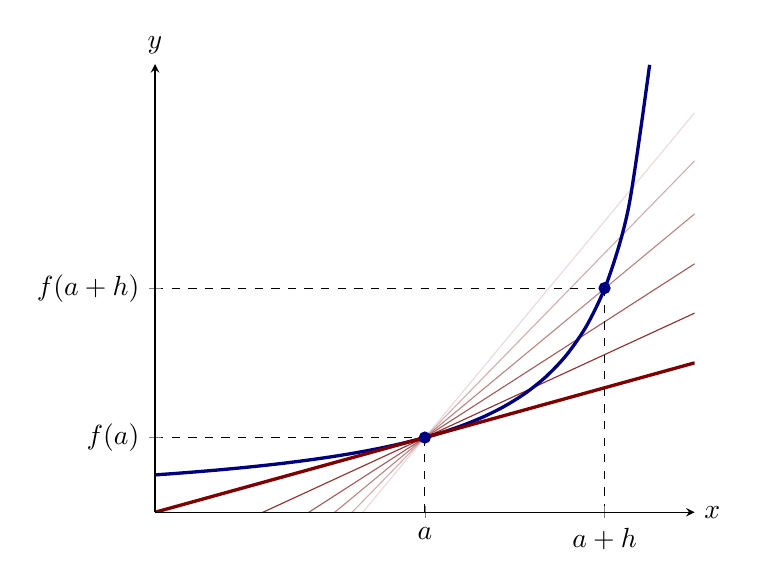
\begin{tikzpicture}
  \begin{axis}[
      domain=0:2, range=0:6,ymax=6,ymin=0,
      axis lines =left, xlabel=$x$, ylabel=$y$,
      every axis y label/.style={at=(current axis.above origin),anchor=south},
      every axis x label/.style={at=(current axis.right of origin),anchor=west},
            xtick={1,1.666}, ytick={1,3},
            xticklabels={$a$,$a+h$}, yticklabels={$f(a)$,$f(a+h)$},
            axis on top,
    ]         
          \addplot [penColor2!15!background, domain=(0:2)] {-3.348+4.348*x};
          \addplot [penColor2!32!background, domain=(0:2)] {-2.704+3.704*x};
          \addplot [penColor2!49!background, domain=(0:2)] {-1.994+2.994*x};         
          \addplot [penColor2!66!background, domain=(0:2)] {-1.326+2.326*x}; 
          \addplot [penColor2!83!background, domain=(0:2)] {-0.666+1.666*x};
	  \addplot [textColor,dashed] plot coordinates {(1,0) (1,1)};
          \addplot [textColor,dashed] plot coordinates {(0,1) (1,1)};
          \addplot [textColor,dashed] plot coordinates {(0,3) (1.666,3)};
          \addplot [textColor,dashed] plot coordinates {(1.666,0) (1.666,3)};
          \addplot [very thick,penColor, smooth,domain=(0:1.833)] {-1/(x-2)};
          \addplot[color=penColor,fill=penColor,only marks,mark=*] coordinates{(1.666,3)};  %% closed hole          
          \addplot[color=penColor,fill=penColor,only marks,mark=*] coordinates{(1,1)};  %% closed hole          
          \addplot [very thick,penColor2, smooth,domain=(0:2)] {x};
        \end{axis}
\end{tikzpicture}
\end{image}
%\todo{This image should be interactive.}


Notice that as $a+h$ approaches $a$, the slopes of the secant lines are approaching
the slope of the tangent line.  This leads to the \textit{definition of the derivative}:

\begin{definition}
  The \dfn{derivative} of $f$ at $a$ is 
  \[
  \eval{\ddx f(x)}_{x=a} = \lim_{h\to 0} \frac{f(a+h) - f(a)}{h}.
  \]
  If this limit exists, then we say that $f$ is \dfn{differentiable}
  at $a$.  If this limit does not exist for a given value of $a$, then
  $f$ is \dfn{non-differentiable} at $a$.
\end{definition}



\begin{question} 
    Which of the following computes the derivative, $\eval{\ddx f(x)}_{x=a}$?
    \begin{selectAll}
      \choice{$\lim_{h\to 0}\frac{(f(a)+h) - f(a)}{(a+h)-a}$}
      \choice[correct]{$\lim_{h\to 0}\frac{f(a+h) - f(a)}{(a+h)-a}$}
      \choice{$\lim_{h\to 0}\frac{(f(a)-h) - f(a)}{(a-h)-a}$}
      \choice[correct]{$\lim_{h\to 0}\frac{f(a-h) - f(a)}{(a-h)-a}$}
      \choice{$\lim_{h\to 0}\frac{f(a) - (f(a)+h)}{a-(a+h)}$}
      \choice[correct]{$\lim_{h\to 0}\frac{f(a) - f(a+h)}{a-(a+h)}$}
      \choice{$\lim_{h\to 0}\frac{f(a) - (f(a)-h)}{a-(a-h)}$}
      \choice[correct]{$\lim_{h\to 0}\frac{f(a) - f(a-h)}{a-(a-h)}$}
    \end{selectAll}
\end{question}

Recalling our original characterization of the slope of the secant line
between $a$ and $x$ which is near by to $a$.  We see that we could also
calculate the derivative of a function by letting $x$ go to $a$.  This 
gives us the following definition:

\begin{definition}
	The \dfn{derivative} of $f$ at $a$ is
	\[
	\eval{\ddx f(x)}_{x=a} = \lim_{x\to a} \frac{f(x) - f(a)}{x-a}.
	\]
\end{definition}

\begin{definition}\index{derivative!notation}
  There are several different notations for the derivative.  The two we'll mainly be using are
  \[
  \eval{\ddx f(x)}_{x=a} = f'(a).
  \]
\end{definition}


Now we will give a number of examples.
\begin{example}
  If $f(x) = x^2-2x$, find the derivative of $f$ at $2$ using the $h\to0$
  characterization.
  \begin{explanation}
    Start with the definition of the derivative,
    \[
    \eval{\ddx f(x)}_{x=2} = \lim_{h\to 0} \frac{f\left(\answer[given]{2+h}\right)-f\left(2\right)}{h}.
    \] 
     Now substitute in for the function we know,
    \[
    \eval{\ddx f(x)}_{x=2} = \lim_{h\to 0}\frac{\answer[given]{(2+h)^2-2(2+h)} -0}{h}.
    \]
    Now expand the numerator of the fraction,
    \[
    \eval{\ddx f(x)}_{x=2} = \lim_{h\to 0} = \frac{4+4h+h^2-4-2h }{h}.
    \]
    Now combine like-terms,
    \[
    \eval{\ddx f(x)}_{x=2} = \lim_{h\to 0}\frac{2h+h^2}{h}.
    \]
    Factor an $h$ from every term in the numerator,
    \[
    \eval{\ddx f(x)}_{x=2} = \lim_{h\to 0}\frac{h\left(\answer[given]{2+h}\right)}{h}.
    \]
    Cancel $h$ from the numerator and denominator,
    \[
    \eval{\ddx f(x)}_{x=2} = \lim_{h\to 0}\answer[given]{2+h}. 
    \]
    Take the limit as $h$ goes to $0$,
    \[
    \eval{\ddx f(x)}_{x=2} = \answer[given]{2}.
    \]
    \begin{onlineOnly}
    For your viewing pleasure, we have below the graph of $y=f(x)$ and the graph of the tangent line at the point $x=2$. 
    \[
    \graph[xmin=-2,xmax=6,ymin=-6,ymax=6]{x^2-2x, 2(x-2)}
    \]
    \end{onlineOnly}
\end{explanation}
\end{example}

\begin{example}
	Find the derivative of $f(x) = x^2+x+1$ at $x=-1$ using the $x\to a$
	characterization.
	\begin{explanation}
		Start with the definition of the derivative,
		\[
		f'(-1) = \lim_{x\to-1}\frac{f\left(x\right)-f\left(\answer[given]{-1}\right)}{x-(-1)}.
		\] 
		Replace $f$ with its formula,
		\[
		f'(-1) = \lim_{x\to-1}\frac{x^2+x+1 - 1}{x+1}.
		\]
		Simplify the top,
		\[
		f'(-1) = \lim_{x\to-1}\frac{x^2+x}{x+1}.
		\]
		Factor,
		\[
		f'(-1) = \lim_{x\to-1}\frac{x\left(\answer[given]{x+1}\right)}{x+1}.
		\]
		Cancel the $x+1$ in the numerator and denominator,
		\[
		f'(-1) = \lim_{x\to-1}x.
		\]
		The expression inside the limit is continuous everywhere, so
		evaluate the limit by plugging in,
		\[
		f'(-1) = \answer[given]{-1}.
		\]
	\end{explanation}
\end{example}

\begin{example}
  Find an equation for the line tangent to $f(x) = \frac{1}{3-x}$ at the point $(2, 1)$.
  \begin{explanation}
    To find an equation for a line, we need two pieces of information.  We need to know
    a point on the line, and we need to know the slope.  In this question, we are given
    that $(2,1)$ is on the line.  That means we need to find the slope of the tangent line.
    Finding the slope of the tangent line at the point $(2,1)$ means finding $f'(2)$.
    
    Start by writing out the definition of the derivative,
    \[
    f'(2) = \lim_{h\to 0} \frac{f(\answer[given]{2+h})-f(2)}{h} = \lim_{h\to 0} \frac{\frac{1}{1-h} - 1}{h}.
    \]
    Multiply by $\frac{1-h}{1-h}$ to clear the fraction in the numerator,
    \[
    f'(2) = \lim_{h\to 0} \frac{\answer[given]{1 - (1-h)}}{h(1-h)}.
    \]
    Combine like-terms in the numerator,
    \[
    f'(2) = \lim_{h\to 0} \frac{h}{h(1-h)},
    \]
    Cancel $h$ from the numerator and denominator,
    \[
    f'(2) = \lim_{h\to 0} \frac{1}{1-h},
    \]		
    Take the limit as $h$ goes to $0$,
    \[
    f'(2) = \answer[given]{1}.
    \]
    We are looking for an equation of the line through the point
    $(2,1)$ with slope $m = f'(2) = 1$.  The point-slope formula tells
    us that the line has equation given by
    \[
    y= \answer[given]{(x-2) + 1}.
    \]
  \begin{onlineOnly}
  We can confirm our results by looking at the graph of $y=f(x)$ and the line $y=(x-2)+1$. 
  \[
  \graph[xmin=-2,xmax=6,ymin=-6,ymax=6]{\frac{1}{3-x}, (x-2)+1}
  \]
  \end{onlineOnly}
  \end{explanation}
\end{example}

\begin{example}
  An object moving along a straight line has displacement given by
  $s(t) = \sqrt{t+3}$.  Find the velocity of the object at time $t=6$.
  \begin{explanation}
    Velocity is the rate of change of displacement with respect to
    time.  We are being asked to find $\eval{\dd{t} s(t)}_{t=6}$.  The
    definition of the derivative gives
    \[
    \eval{\dd{t} s(t)}_{t=6} = \lim_{h \to 0} \frac{s(\answer[given]{6+h})-s(6)}{h} = \lim_{h\to 0} \frac{\sqrt{\answer[given]{9+h}}-3}{h}.
    \]
    Multiply by $\frac{\sqrt{9+h}+3}{\sqrt{9+h}+3}$,
    \[
    \eval{\dd{t} s(t)}_{t=6} = \lim_{h\to 0} \left(\frac{\sqrt{9+h}-3}{h} \right)\left( \frac{\sqrt{9+h}+3}{\sqrt{9+h}+3} \right).
    \]		
    Now expand the numerator,
    \[
    \eval{\dd{t} s(t)}_{t=6} = \lim_{h \to 0} \frac{\answer[given]{9+h} - 9}{h\left(\sqrt{9+h}+3 \right)}.
    \]
    Combine like-terms,
    \[
    \eval{\dd{t} s(t)}_{t=6} = \lim_{h \to 0} \frac{\answer[given]{h}}{h\left(\sqrt{9+h}+3\right)}.
    \]
    Cancel $h$ from the numerator and denominator,
    \[
    \eval{\dd{t} s(t)}_{t=6} = \lim_{h\to 0} \frac{1}{\sqrt{9+h}+3}.
    \]
    Take the limit as $h$ tends to $0$,
    \[
    \eval{\dd{t} s(t)}_{t=6} = \answer[given]{\frac{1}{6}}.
    \]
    The object has velocity $\answer[given]{\frac{1}{6}}$ at time $t=6$.
	\begin{onlineOnly}
	Below we can see the graph of $y=s(t)$ and the tangent line at $t=6$, with a slope of $\frac{1}{6}$. 
	\[
	\graph[xmin=-1,xmax=15,ymin=-8,ymax=8]{\sqrt{x+3}, \frac{1}{6}(x-6)+3}
	\]
	\end{onlineOnly}
	\end{explanation}
\end{example}







\end{document}
